\documentclass[11pt]{article}
\usepackage[textwidth=18.0cm, textheight=23.0cm, top=2.0cm]{geometry}
\usepackage{pst-all}
\usepackage{amssymb}
\usepackage{tikz}
\usepackage{underscore}\begin{document}
\pagestyle{empty}


ClassName: \underline{\textbf{Class_10.2bp-46}}
\par
BinSize: \underline{\textbf{100 × 100}}
\par
ReduceSize: \underline{\textbf{100 × 100}}
\par
TypeNum: \underline{\textbf{99}}
\par
Num: \underline{\textbf{100}}
\par
OutS: \underline{\textbf{140000}}
\par
InS: \underline{\textbf{128538}}
\par
Rate: \underline{\textbf{0.918}}
\par
UB: \underline{\textbf{14}}
\par
LB0: \underline{\textbf{13}}
\par
LB: \underline{\textbf{14}}
\par
LBWithCut: \underline{\textbf{14}}
\par
NodeCut: \underline{\textbf{0}}
\par
ExtendedNodeCnt: \underline{\textbf{1}}
\par
GenNodeCnt: \underline{\textbf{1}}
\par
PrimalNode: \underline{\textbf{0}}
\par
ColumnCount: \underline{\textbf{69}}
\par
TotalCutCount: \underline{\textbf{0}}
\par
RootCutCount: \underline{\textbf{0}}
\par
LPSolverCnt: \underline{\textbf{55}}
\par
PricingSolverCnt: \underline{\textbf{55}}
\par
BranchAndBoundNum: \underline{\textbf{1}}
\par
isOpt: \underline{\textbf{false}}
\par
TimeOnPrimal: \underline{\textbf{0.000 s}}
\par
TimeOnPricing: \underline{\textbf{3600.340 s}}
\par
TimeOnRmp: \underline{\textbf{0.125 s}}
\par
TotalTime: \underline{\textbf{3600.516 s}}
\par
\newpage


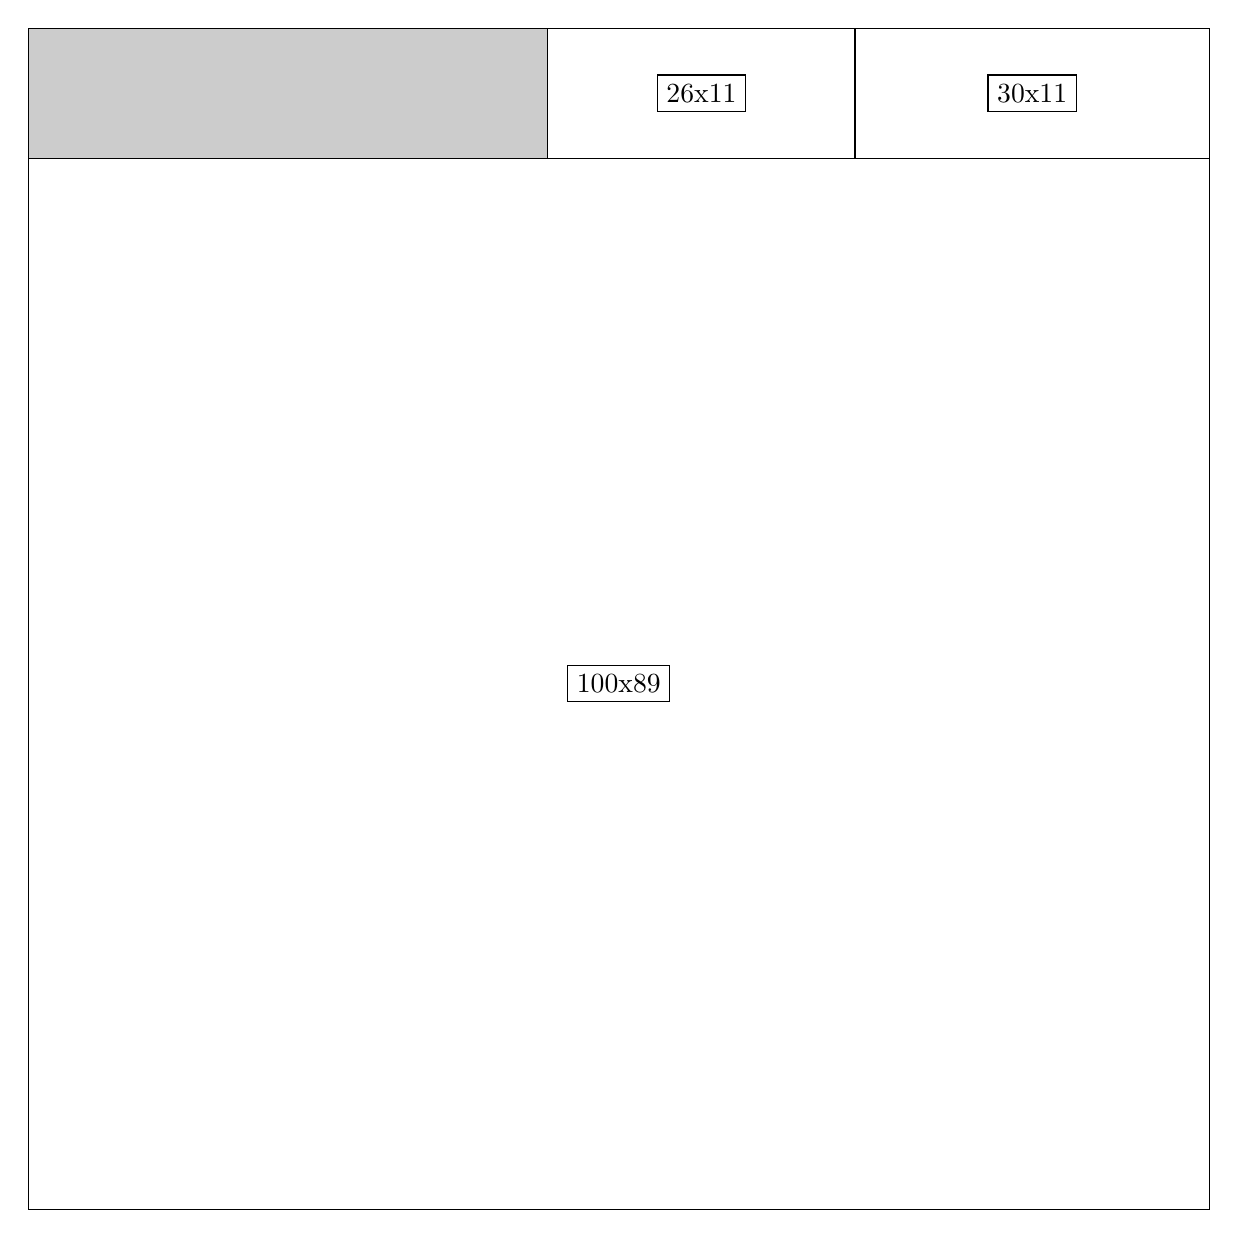
\begin{tikzpicture}[shorten >=1pt,scale=1.0,every node/.style={scale=1.0},->]
\tikzstyle{vertex}=[circle,fill=black!25,minimum size=14pt,inner sep=0pt]
\filldraw[fill=gray!40!white, draw=black] (0,0) rectangle (15.0,15.0);
\foreach \name/\x/\y/\w/\h in {100x89/0.0/0.0/15.0/13.35,30x11/10.5/13.35/4.5/1.65,26x11/6.6/13.35/3.9/1.65}
\filldraw[fill=white!40!white, draw=black] (\x,\y) rectangle node[draw] (\name) {\name} ++(\w,\h);
\end{tikzpicture}


w =100 , h =89 , x =0 , y =0 , v =8900
\par
w =30 , h =11 , x =70 , y =89 , v =330
\par
w =26 , h =11 , x =44 , y =89 , v =286
\par
\newpage


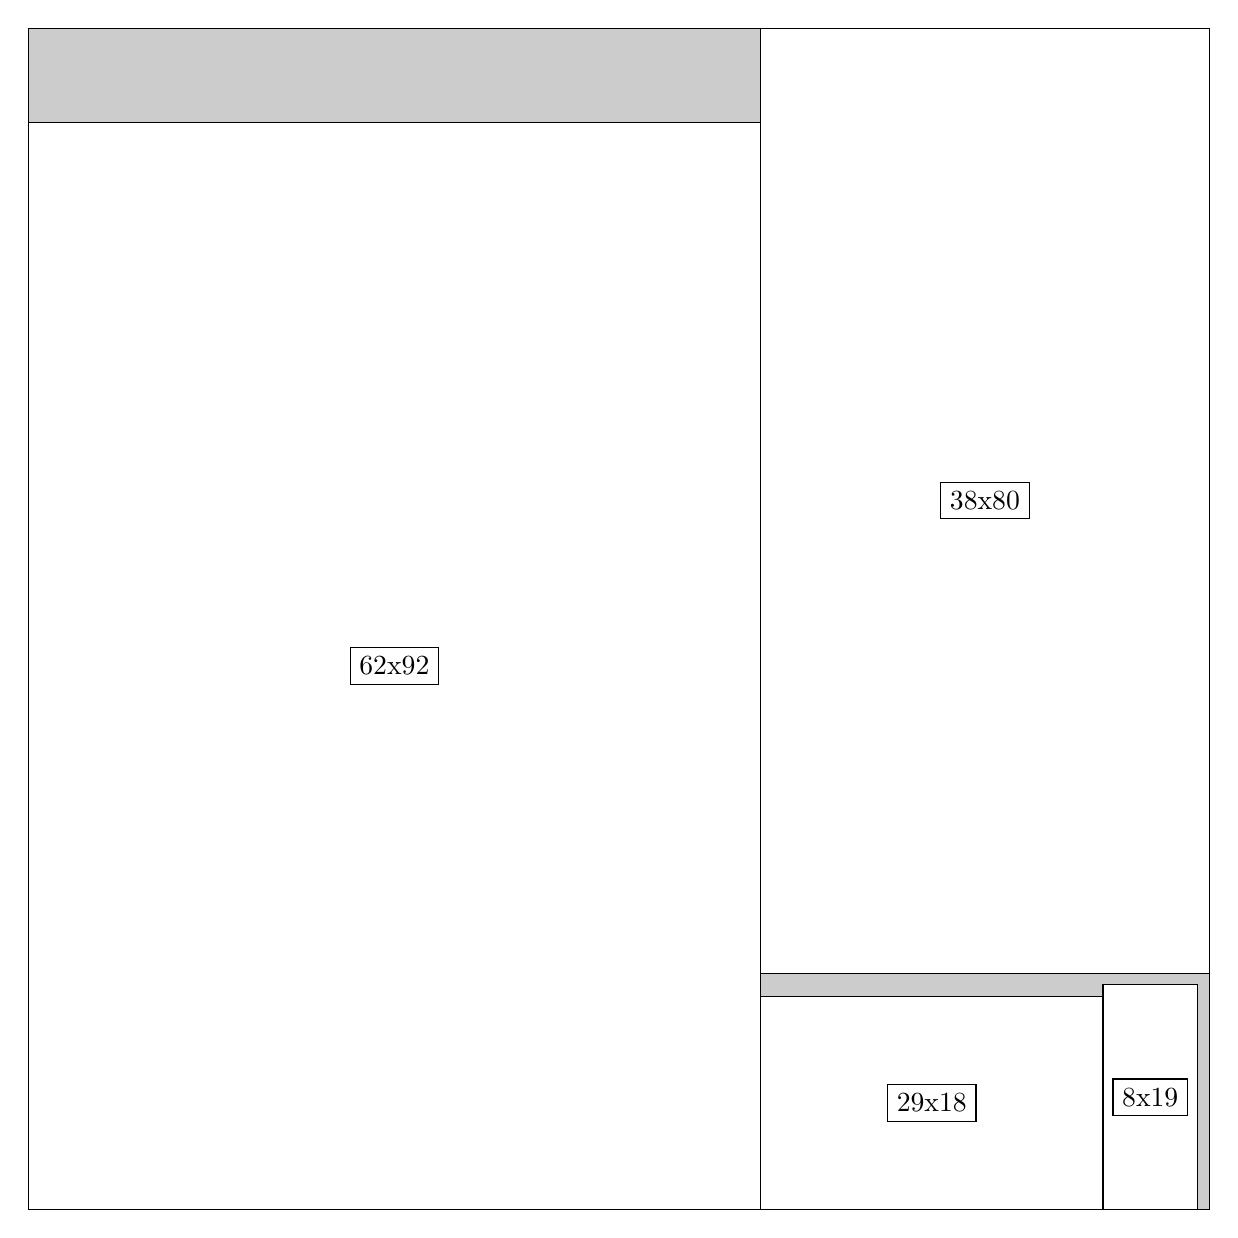
\begin{tikzpicture}[shorten >=1pt,scale=1.0,every node/.style={scale=1.0},->]
\tikzstyle{vertex}=[circle,fill=black!25,minimum size=14pt,inner sep=0pt]
\filldraw[fill=gray!40!white, draw=black] (0,0) rectangle (15.0,15.0);
\foreach \name/\x/\y/\w/\h in {62x92/0.0/0.0/9.299999999999999/13.799999999999999,38x80/9.299999999999999/3.0/5.7/12.0,29x18/9.299999999999999/0.0/4.35/2.6999999999999997,8x19/13.65/0.0/1.2/2.85}
\filldraw[fill=white!40!white, draw=black] (\x,\y) rectangle node[draw] (\name) {\name} ++(\w,\h);
\end{tikzpicture}


w =62 , h =92 , x =0 , y =0 , v =5704
\par
w =38 , h =80 , x =62 , y =20 , v =3040
\par
w =29 , h =18 , x =62 , y =0 , v =522
\par
w =8 , h =19 , x =91 , y =0 , v =152
\par
\newpage


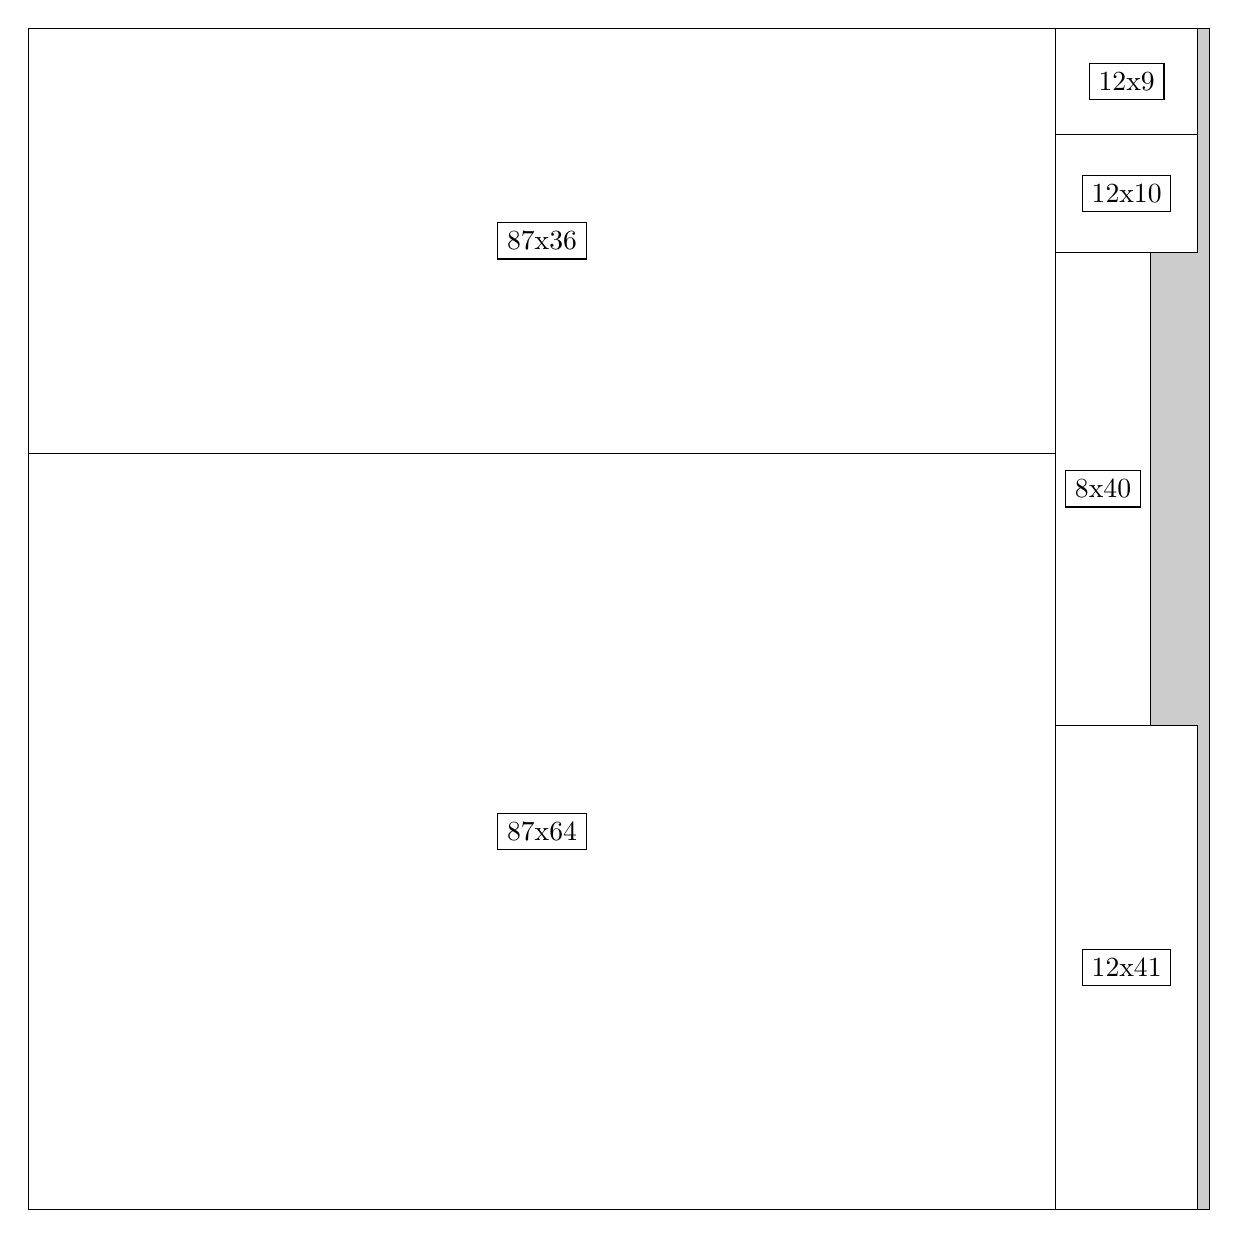
\begin{tikzpicture}[shorten >=1pt,scale=1.0,every node/.style={scale=1.0},->]
\tikzstyle{vertex}=[circle,fill=black!25,minimum size=14pt,inner sep=0pt]
\filldraw[fill=gray!40!white, draw=black] (0,0) rectangle (15.0,15.0);
\foreach \name/\x/\y/\w/\h in {87x64/0.0/0.0/13.049999999999999/9.6,87x36/0.0/9.6/13.049999999999999/5.3999999999999995,12x41/13.049999999999999/0.0/1.7999999999999998/6.1499999999999995,8x40/13.049999999999999/6.1499999999999995/1.2/6.0,12x10/13.049999999999999/12.15/1.7999999999999998/1.5,12x9/13.049999999999999/13.65/1.7999999999999998/1.3499999999999999}
\filldraw[fill=white!40!white, draw=black] (\x,\y) rectangle node[draw] (\name) {\name} ++(\w,\h);
\end{tikzpicture}


w =87 , h =64 , x =0 , y =0 , v =5568
\par
w =87 , h =36 , x =0 , y =64 , v =3132
\par
w =12 , h =41 , x =87 , y =0 , v =492
\par
w =8 , h =40 , x =87 , y =41 , v =320
\par
w =12 , h =10 , x =87 , y =81 , v =120
\par
w =12 , h =9 , x =87 , y =91 , v =108
\par
\newpage


\begin{tikzpicture}[shorten >=1pt,scale=1.0,every node/.style={scale=1.0},->]
\tikzstyle{vertex}=[circle,fill=black!25,minimum size=14pt,inner sep=0pt]
\filldraw[fill=gray!40!white, draw=black] (0,0) rectangle (15.0,15.0);
\foreach \name/\x/\y/\w/\h in {75x68/0.0/0.0/11.25/10.2,22x72/11.25/0.6/3.3/10.799999999999999,31x32/6.6/10.2/4.6499999999999995/4.8,44x18/0.0/10.2/6.6/2.6999999999999997,22x24/11.25/11.4/3.3/3.5999999999999996,3x96/14.549999999999999/0.6/0.44999999999999996/14.399999999999999,41x4/0.0/12.9/6.1499999999999995/0.6,17x8/3.5999999999999996/13.799999999999999/2.55/1.2,14x8/1.5/13.799999999999999/2.1/1.2,25x4/11.25/0.0/3.75/0.6,41x2/0.0/13.5/6.1499999999999995/0.3,3x14/6.1499999999999995/12.9/0.44999999999999996/2.1,4x8/0.8999999999999999/13.799999999999999/0.6/1.2,4x7/0.0/13.799999999999999/0.6/1.05}
\filldraw[fill=white!40!white, draw=black] (\x,\y) rectangle node[draw] (\name) {\name} ++(\w,\h);
\end{tikzpicture}


w =75 , h =68 , x =0 , y =0 , v =5100
\par
w =22 , h =72 , x =75 , y =4 , v =1584
\par
w =31 , h =32 , x =44 , y =68 , v =992
\par
w =44 , h =18 , x =0 , y =68 , v =792
\par
w =22 , h =24 , x =75 , y =76 , v =528
\par
w =3 , h =96 , x =97 , y =4 , v =288
\par
w =41 , h =4 , x =0 , y =86 , v =164
\par
w =17 , h =8 , x =24 , y =92 , v =136
\par
w =14 , h =8 , x =10 , y =92 , v =112
\par
w =25 , h =4 , x =75 , y =0 , v =100
\par
w =41 , h =2 , x =0 , y =90 , v =82
\par
w =3 , h =14 , x =41 , y =86 , v =42
\par
w =4 , h =8 , x =6 , y =92 , v =32
\par
w =4 , h =7 , x =0 , y =92 , v =28
\par
\newpage


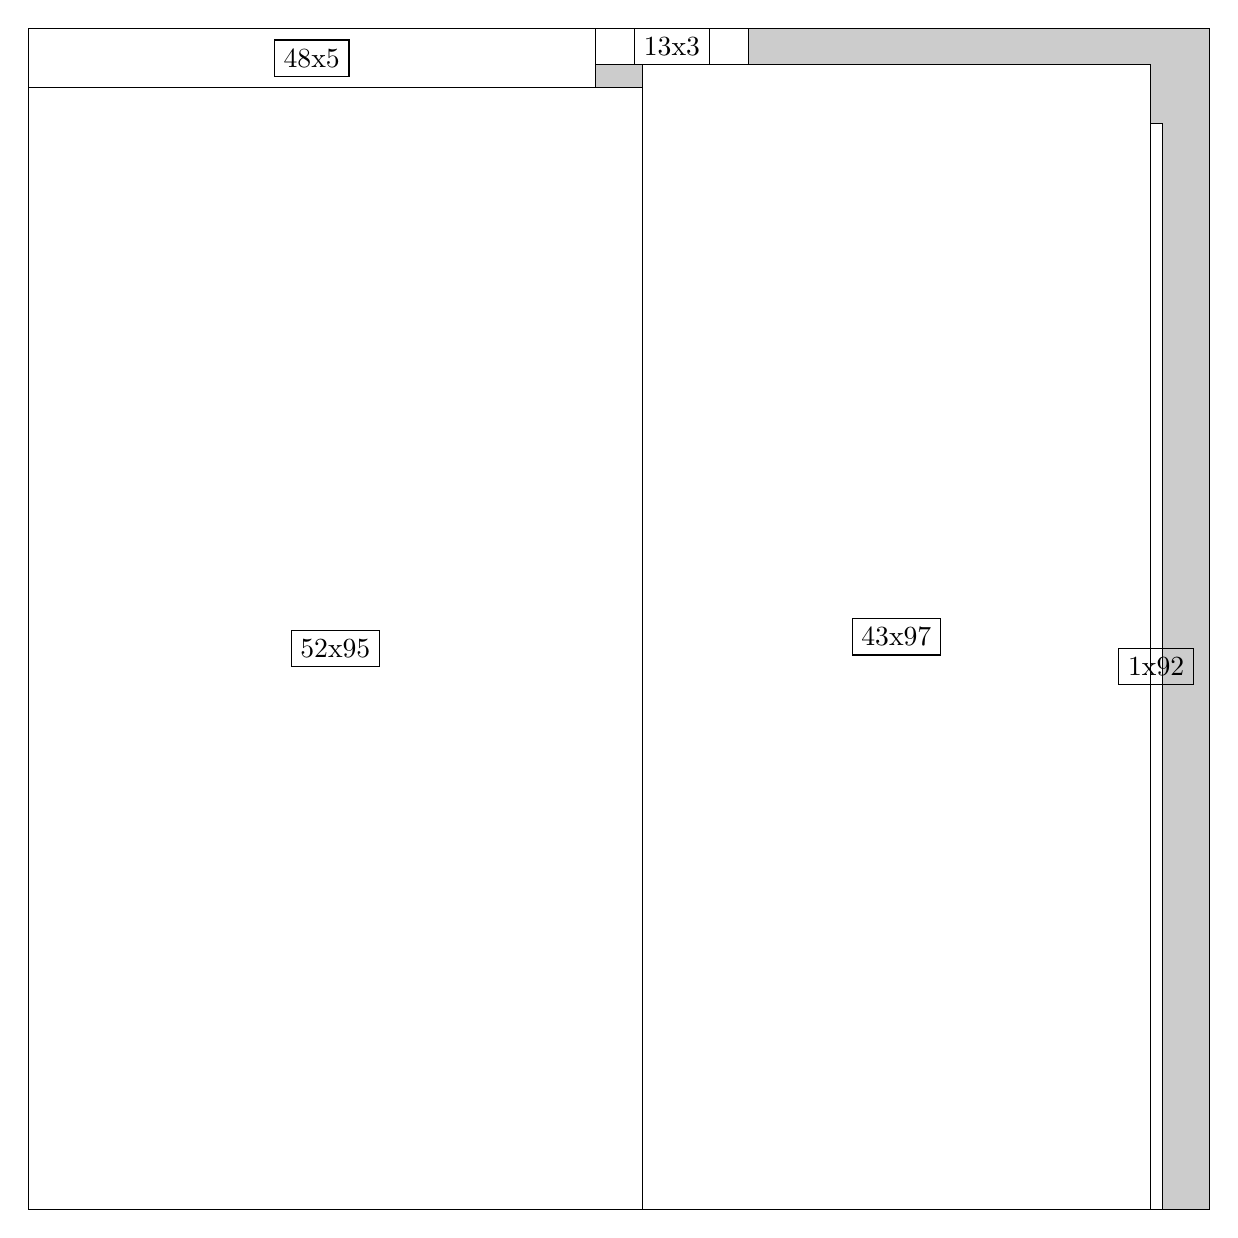
\begin{tikzpicture}[shorten >=1pt,scale=1.0,every node/.style={scale=1.0},->]
\tikzstyle{vertex}=[circle,fill=black!25,minimum size=14pt,inner sep=0pt]
\filldraw[fill=gray!40!white, draw=black] (0,0) rectangle (15.0,15.0);
\foreach \name/\x/\y/\w/\h in {52x95/0.0/0.0/7.8/14.25,43x97/7.8/0.0/6.45/14.549999999999999,48x5/0.0/14.25/7.199999999999999/0.75,1x92/14.25/0.0/0.15/13.799999999999999,13x3/7.199999999999999/14.549999999999999/1.95/0.44999999999999996}
\filldraw[fill=white!40!white, draw=black] (\x,\y) rectangle node[draw] (\name) {\name} ++(\w,\h);
\end{tikzpicture}


w =52 , h =95 , x =0 , y =0 , v =4940
\par
w =43 , h =97 , x =52 , y =0 , v =4171
\par
w =48 , h =5 , x =0 , y =95 , v =240
\par
w =1 , h =92 , x =95 , y =0 , v =92
\par
w =13 , h =3 , x =48 , y =97 , v =39
\par
\newpage


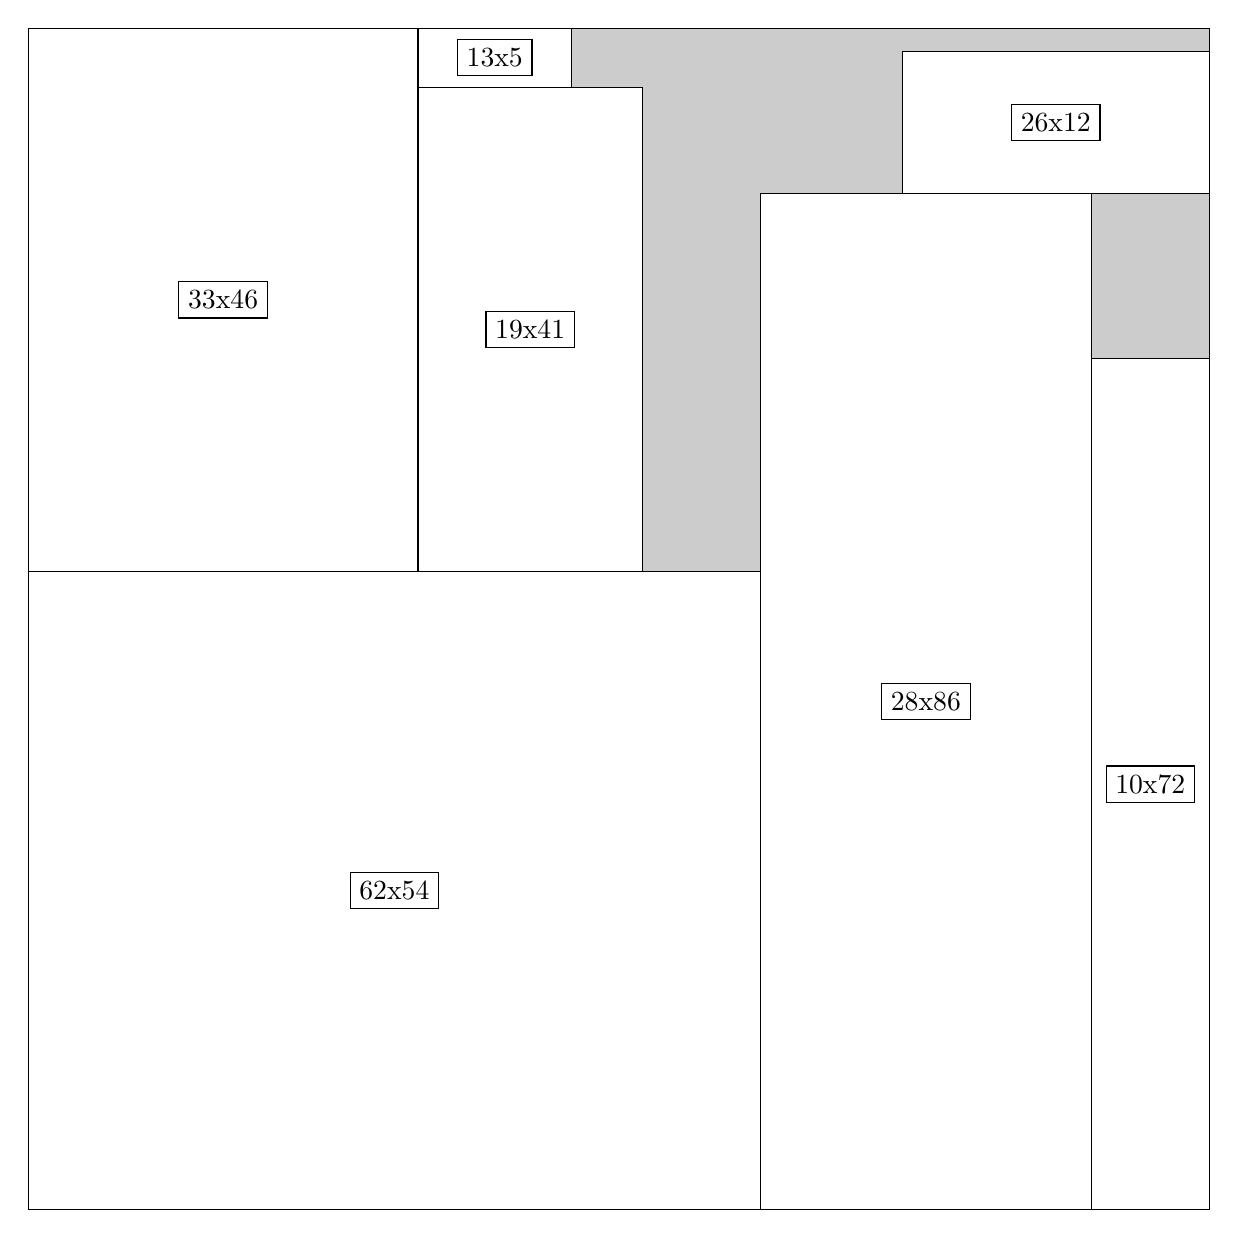
\begin{tikzpicture}[shorten >=1pt,scale=1.0,every node/.style={scale=1.0},->]
\tikzstyle{vertex}=[circle,fill=black!25,minimum size=14pt,inner sep=0pt]
\filldraw[fill=gray!40!white, draw=black] (0,0) rectangle (15.0,15.0);
\foreach \name/\x/\y/\w/\h in {10x72/13.5/0.0/1.5/10.799999999999999,28x86/9.299999999999999/0.0/4.2/12.9,33x46/0.0/8.1/4.95/6.8999999999999995,19x41/4.95/8.1/2.85/6.1499999999999995,62x54/0.0/0.0/9.299999999999999/8.1,26x12/11.1/12.9/3.9/1.7999999999999998,13x5/4.95/14.25/1.95/0.75}
\filldraw[fill=white!40!white, draw=black] (\x,\y) rectangle node[draw] (\name) {\name} ++(\w,\h);
\end{tikzpicture}


w =10 , h =72 , x =90 , y =0 , v =720
\par
w =28 , h =86 , x =62 , y =0 , v =2408
\par
w =33 , h =46 , x =0 , y =54 , v =1518
\par
w =19 , h =41 , x =33 , y =54 , v =779
\par
w =62 , h =54 , x =0 , y =0 , v =3348
\par
w =26 , h =12 , x =74 , y =86 , v =312
\par
w =13 , h =5 , x =33 , y =95 , v =65
\par
\newpage


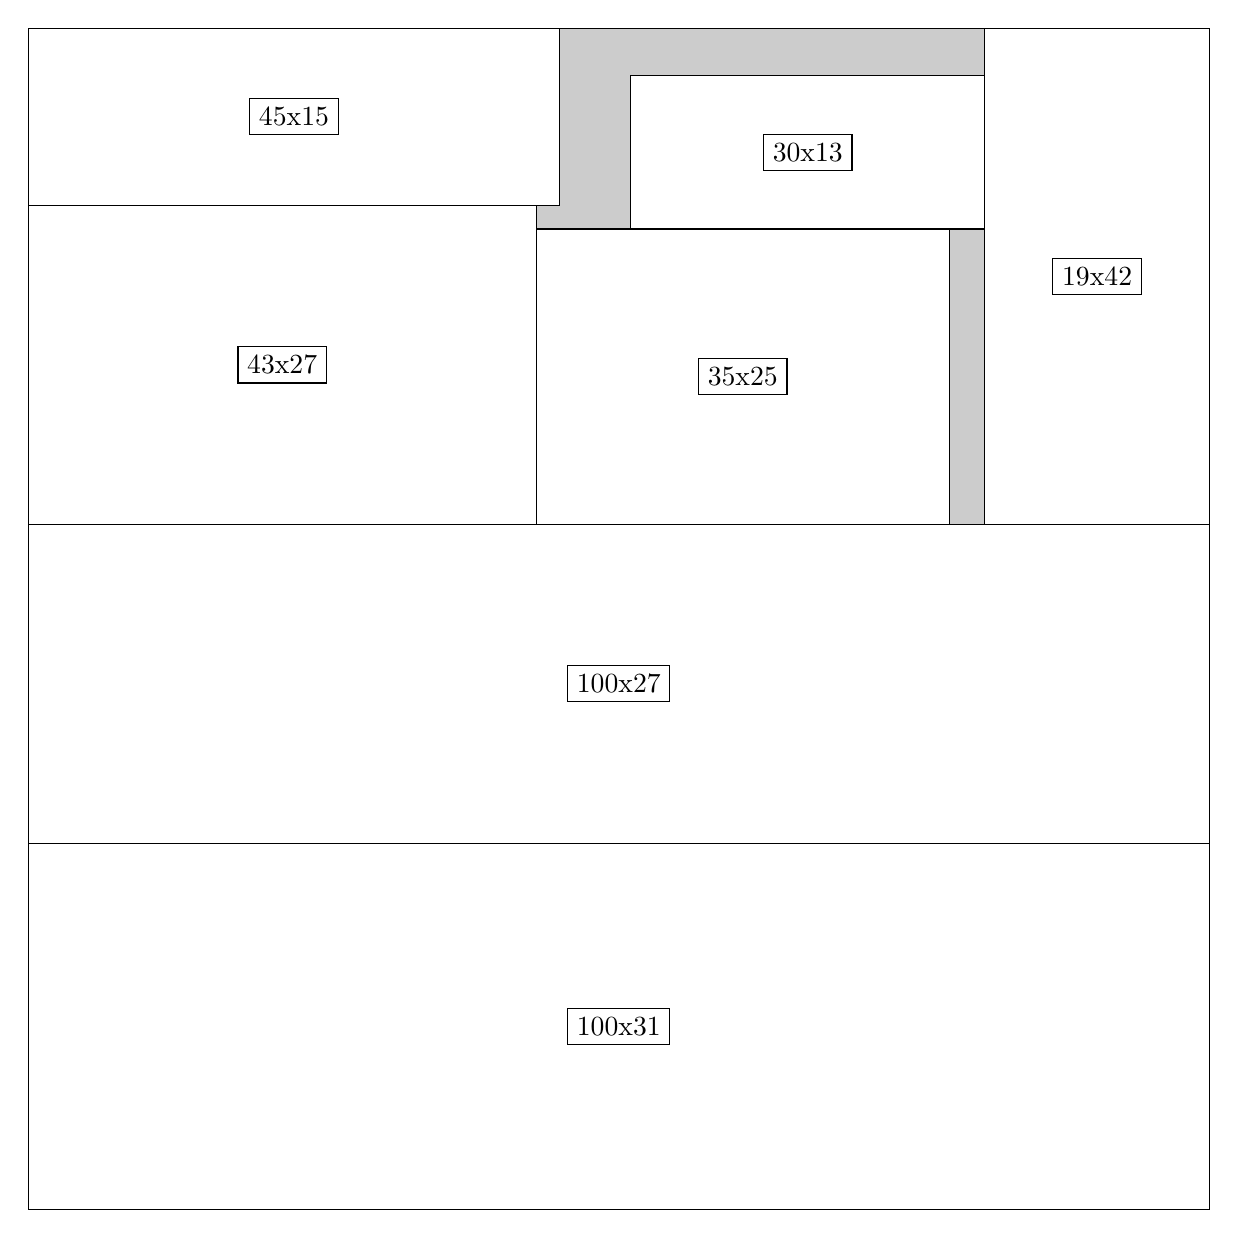
\begin{tikzpicture}[shorten >=1pt,scale=1.0,every node/.style={scale=1.0},->]
\tikzstyle{vertex}=[circle,fill=black!25,minimum size=14pt,inner sep=0pt]
\filldraw[fill=gray!40!white, draw=black] (0,0) rectangle (15.0,15.0);
\foreach \name/\x/\y/\w/\h in {100x31/0.0/0.0/15.0/4.6499999999999995,100x27/0.0/4.6499999999999995/15.0/4.05,43x27/0.0/8.7/6.45/4.05,35x25/6.45/8.7/5.25/3.75,19x42/12.15/8.7/2.85/6.3,45x15/0.0/12.75/6.75/2.25,30x13/7.6499999999999995/12.45/4.5/1.95}
\filldraw[fill=white!40!white, draw=black] (\x,\y) rectangle node[draw] (\name) {\name} ++(\w,\h);
\end{tikzpicture}


w =100 , h =31 , x =0 , y =0 , v =3100
\par
w =100 , h =27 , x =0 , y =31 , v =2700
\par
w =43 , h =27 , x =0 , y =58 , v =1161
\par
w =35 , h =25 , x =43 , y =58 , v =875
\par
w =19 , h =42 , x =81 , y =58 , v =798
\par
w =45 , h =15 , x =0 , y =85 , v =675
\par
w =30 , h =13 , x =51 , y =83 , v =390
\par
\newpage


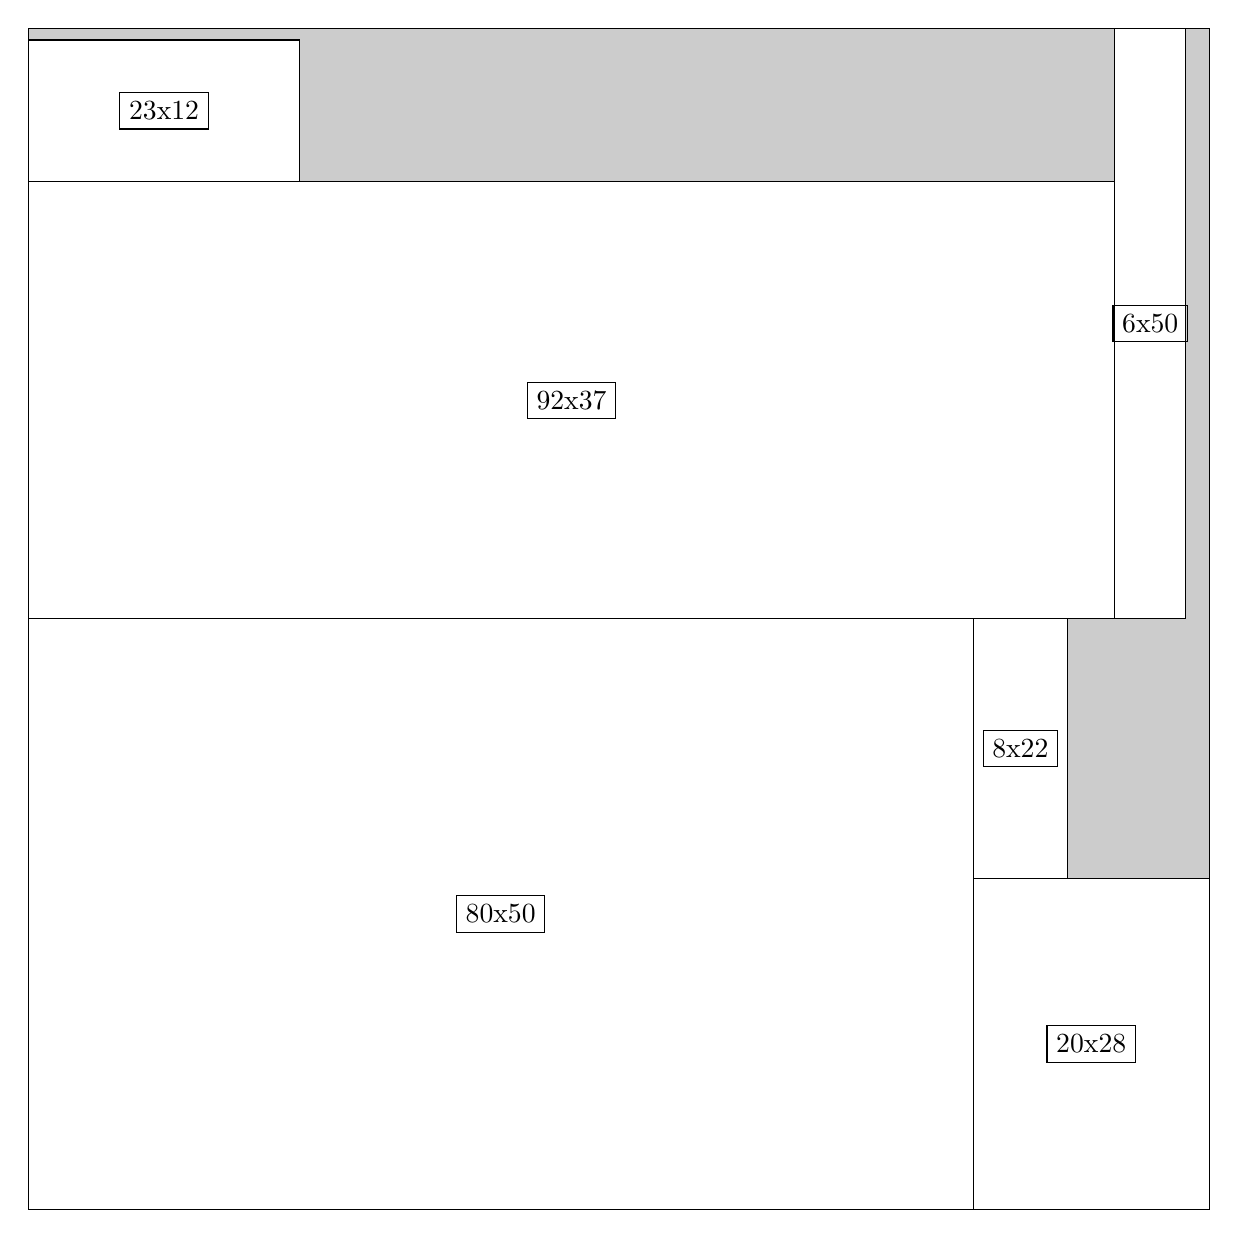
\begin{tikzpicture}[shorten >=1pt,scale=1.0,every node/.style={scale=1.0},->]
\tikzstyle{vertex}=[circle,fill=black!25,minimum size=14pt,inner sep=0pt]
\filldraw[fill=gray!40!white, draw=black] (0,0) rectangle (15.0,15.0);
\foreach \name/\x/\y/\w/\h in {80x50/0.0/0.0/12.0/7.5,92x37/0.0/7.5/13.799999999999999/5.55,20x28/12.0/0.0/3.0/4.2,6x50/13.799999999999999/7.5/0.8999999999999999/7.5,23x12/0.0/13.049999999999999/3.4499999999999997/1.7999999999999998,8x22/12.0/4.2/1.2/3.3}
\filldraw[fill=white!40!white, draw=black] (\x,\y) rectangle node[draw] (\name) {\name} ++(\w,\h);
\end{tikzpicture}


w =80 , h =50 , x =0 , y =0 , v =4000
\par
w =92 , h =37 , x =0 , y =50 , v =3404
\par
w =20 , h =28 , x =80 , y =0 , v =560
\par
w =6 , h =50 , x =92 , y =50 , v =300
\par
w =23 , h =12 , x =0 , y =87 , v =276
\par
w =8 , h =22 , x =80 , y =28 , v =176
\par
\newpage


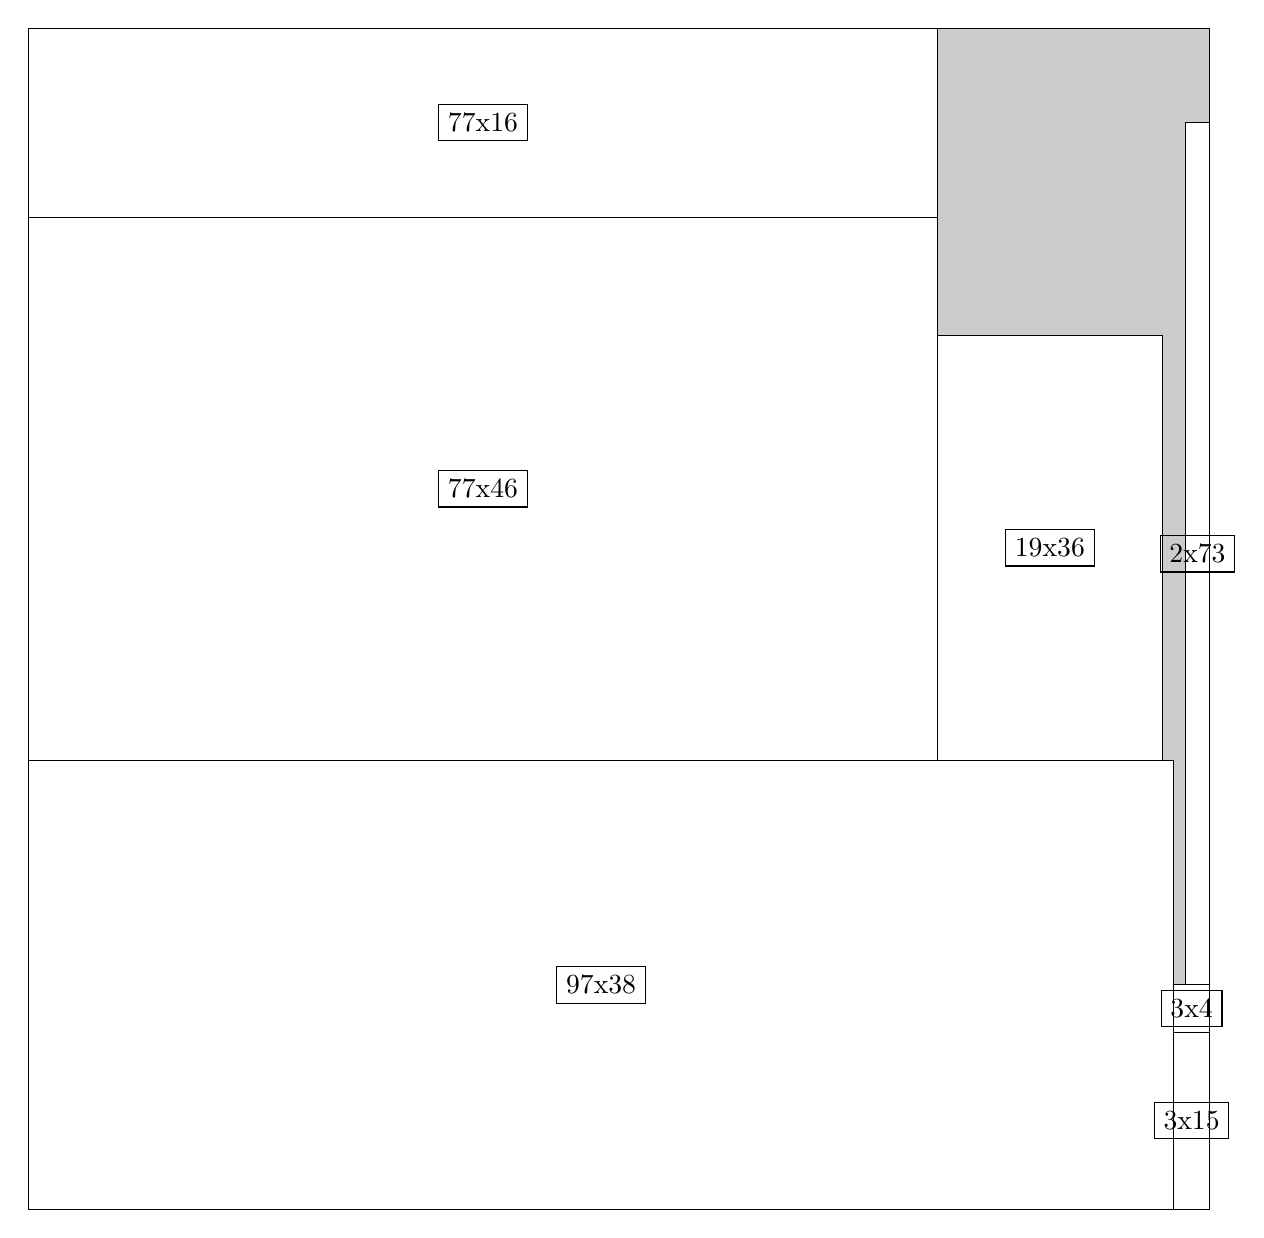
\begin{tikzpicture}[shorten >=1pt,scale=1.0,every node/.style={scale=1.0},->]
\tikzstyle{vertex}=[circle,fill=black!25,minimum size=14pt,inner sep=0pt]
\filldraw[fill=gray!40!white, draw=black] (0,0) rectangle (15.0,15.0);
\foreach \name/\x/\y/\w/\h in {97x38/0.0/0.0/14.549999999999999/5.7,77x46/0.0/5.7/11.549999999999999/6.8999999999999995,77x16/0.0/12.6/11.549999999999999/2.4,19x36/11.549999999999999/5.7/2.85/5.3999999999999995,2x73/14.7/2.85/0.3/10.95,3x15/14.549999999999999/0.0/0.44999999999999996/2.25,3x4/14.549999999999999/2.25/0.44999999999999996/0.6}
\filldraw[fill=white!40!white, draw=black] (\x,\y) rectangle node[draw] (\name) {\name} ++(\w,\h);
\end{tikzpicture}


w =97 , h =38 , x =0 , y =0 , v =3686
\par
w =77 , h =46 , x =0 , y =38 , v =3542
\par
w =77 , h =16 , x =0 , y =84 , v =1232
\par
w =19 , h =36 , x =77 , y =38 , v =684
\par
w =2 , h =73 , x =98 , y =19 , v =146
\par
w =3 , h =15 , x =97 , y =0 , v =45
\par
w =3 , h =4 , x =97 , y =15 , v =12
\par
\newpage


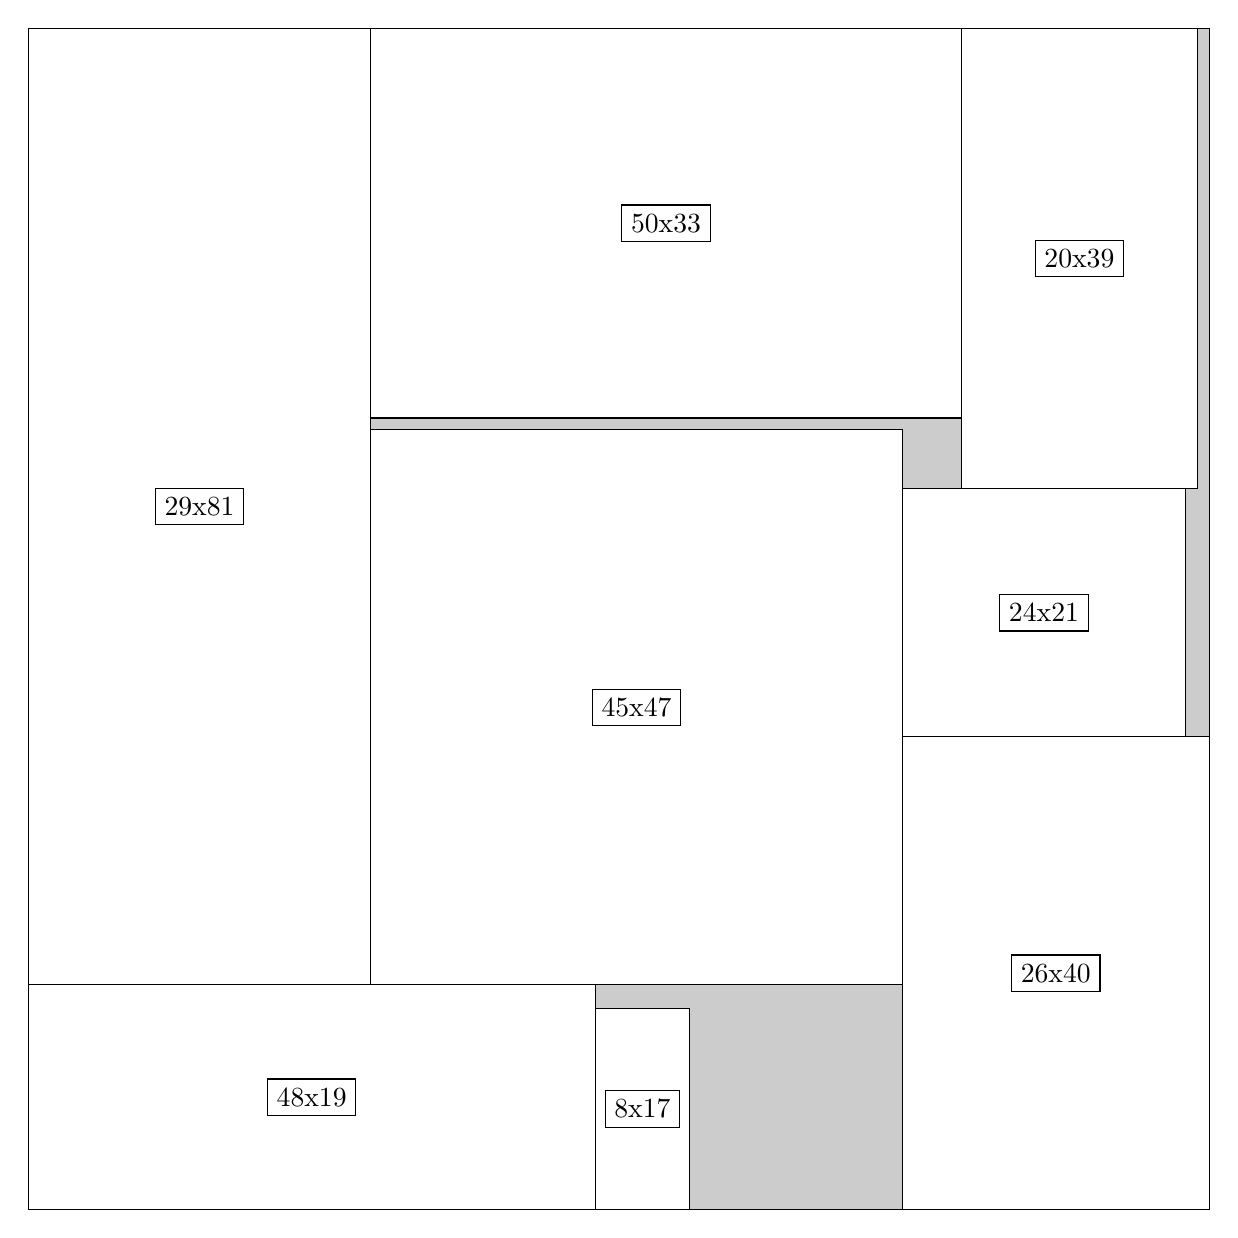
\begin{tikzpicture}[shorten >=1pt,scale=1.0,every node/.style={scale=1.0},->]
\tikzstyle{vertex}=[circle,fill=black!25,minimum size=14pt,inner sep=0pt]
\filldraw[fill=gray!40!white, draw=black] (0,0) rectangle (15.0,15.0);
\foreach \name/\x/\y/\w/\h in {48x19/0.0/0.0/7.199999999999999/2.85,45x47/4.35/2.85/6.75/7.05,50x33/4.35/10.049999999999999/7.5/4.95,26x40/11.1/0.0/3.9/6.0,29x81/0.0/2.85/4.35/12.15,20x39/11.85/9.15/3.0/5.85,24x21/11.1/6.0/3.5999999999999996/3.15,8x17/7.199999999999999/0.0/1.2/2.55}
\filldraw[fill=white!40!white, draw=black] (\x,\y) rectangle node[draw] (\name) {\name} ++(\w,\h);
\end{tikzpicture}


w =48 , h =19 , x =0 , y =0 , v =912
\par
w =45 , h =47 , x =29 , y =19 , v =2115
\par
w =50 , h =33 , x =29 , y =67 , v =1650
\par
w =26 , h =40 , x =74 , y =0 , v =1040
\par
w =29 , h =81 , x =0 , y =19 , v =2349
\par
w =20 , h =39 , x =79 , y =61 , v =780
\par
w =24 , h =21 , x =74 , y =40 , v =504
\par
w =8 , h =17 , x =48 , y =0 , v =136
\par
\newpage


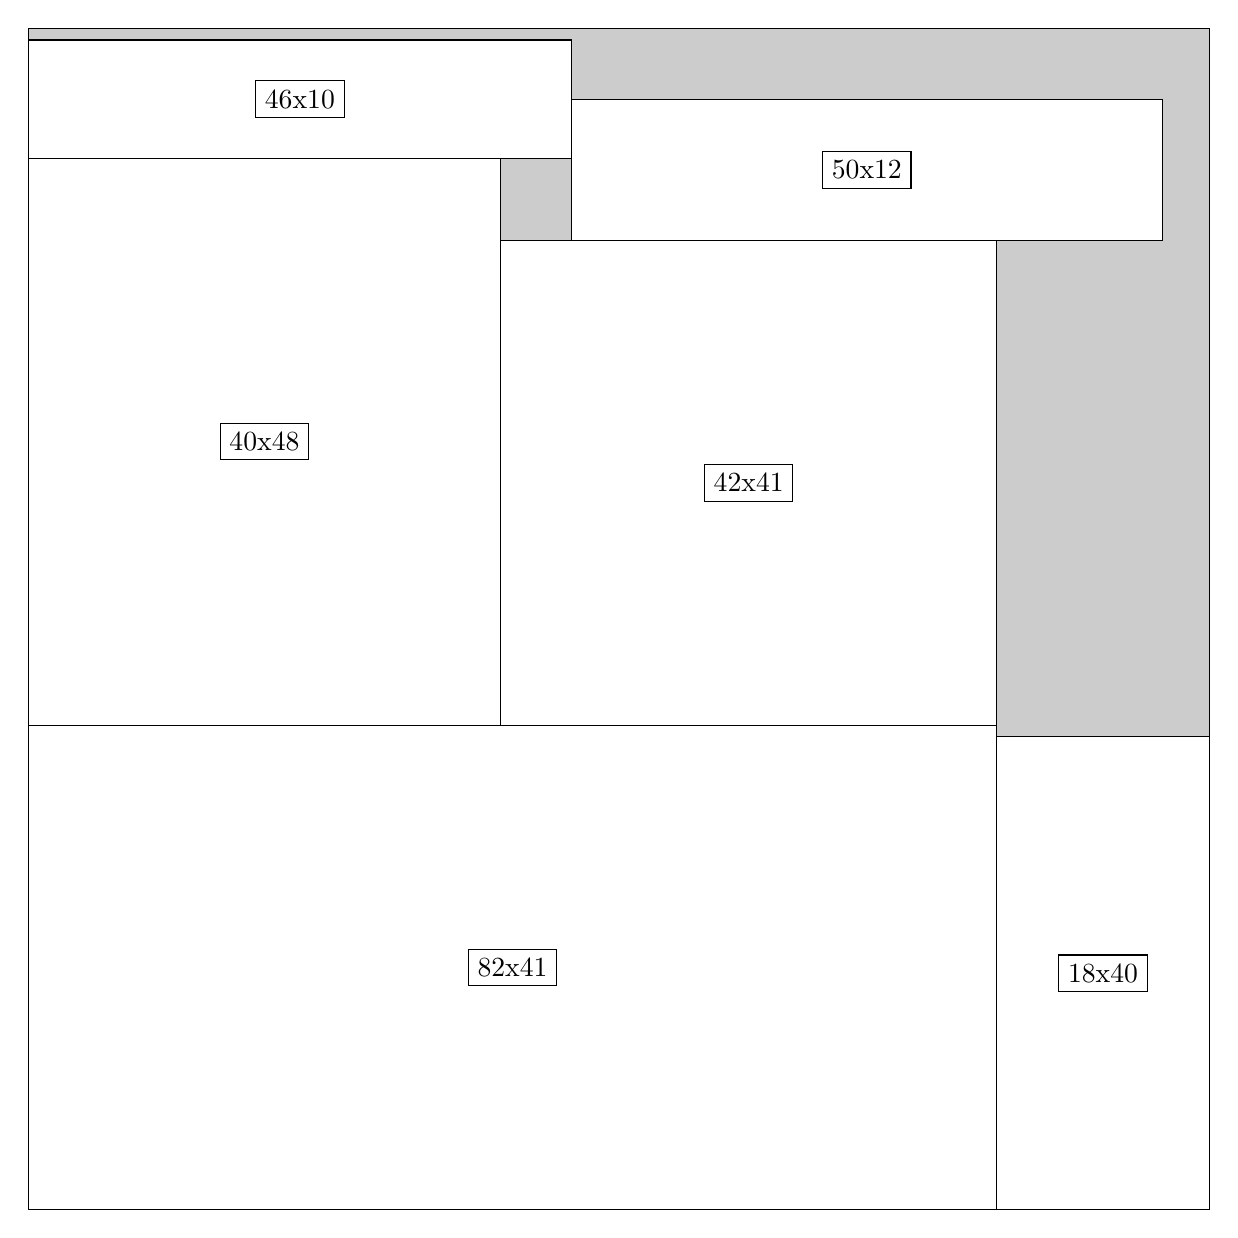
\begin{tikzpicture}[shorten >=1pt,scale=1.0,every node/.style={scale=1.0},->]
\tikzstyle{vertex}=[circle,fill=black!25,minimum size=14pt,inner sep=0pt]
\filldraw[fill=gray!40!white, draw=black] (0,0) rectangle (15.0,15.0);
\foreach \name/\x/\y/\w/\h in {82x41/0.0/0.0/12.299999999999999/6.1499999999999995,40x48/0.0/6.1499999999999995/6.0/7.199999999999999,42x41/6.0/6.1499999999999995/6.3/6.1499999999999995,18x40/12.299999999999999/0.0/2.6999999999999997/6.0,50x12/6.8999999999999995/12.299999999999999/7.5/1.7999999999999998,46x10/0.0/13.35/6.8999999999999995/1.5}
\filldraw[fill=white!40!white, draw=black] (\x,\y) rectangle node[draw] (\name) {\name} ++(\w,\h);
\end{tikzpicture}


w =82 , h =41 , x =0 , y =0 , v =3362
\par
w =40 , h =48 , x =0 , y =41 , v =1920
\par
w =42 , h =41 , x =40 , y =41 , v =1722
\par
w =18 , h =40 , x =82 , y =0 , v =720
\par
w =50 , h =12 , x =46 , y =82 , v =600
\par
w =46 , h =10 , x =0 , y =89 , v =460
\par
\newpage


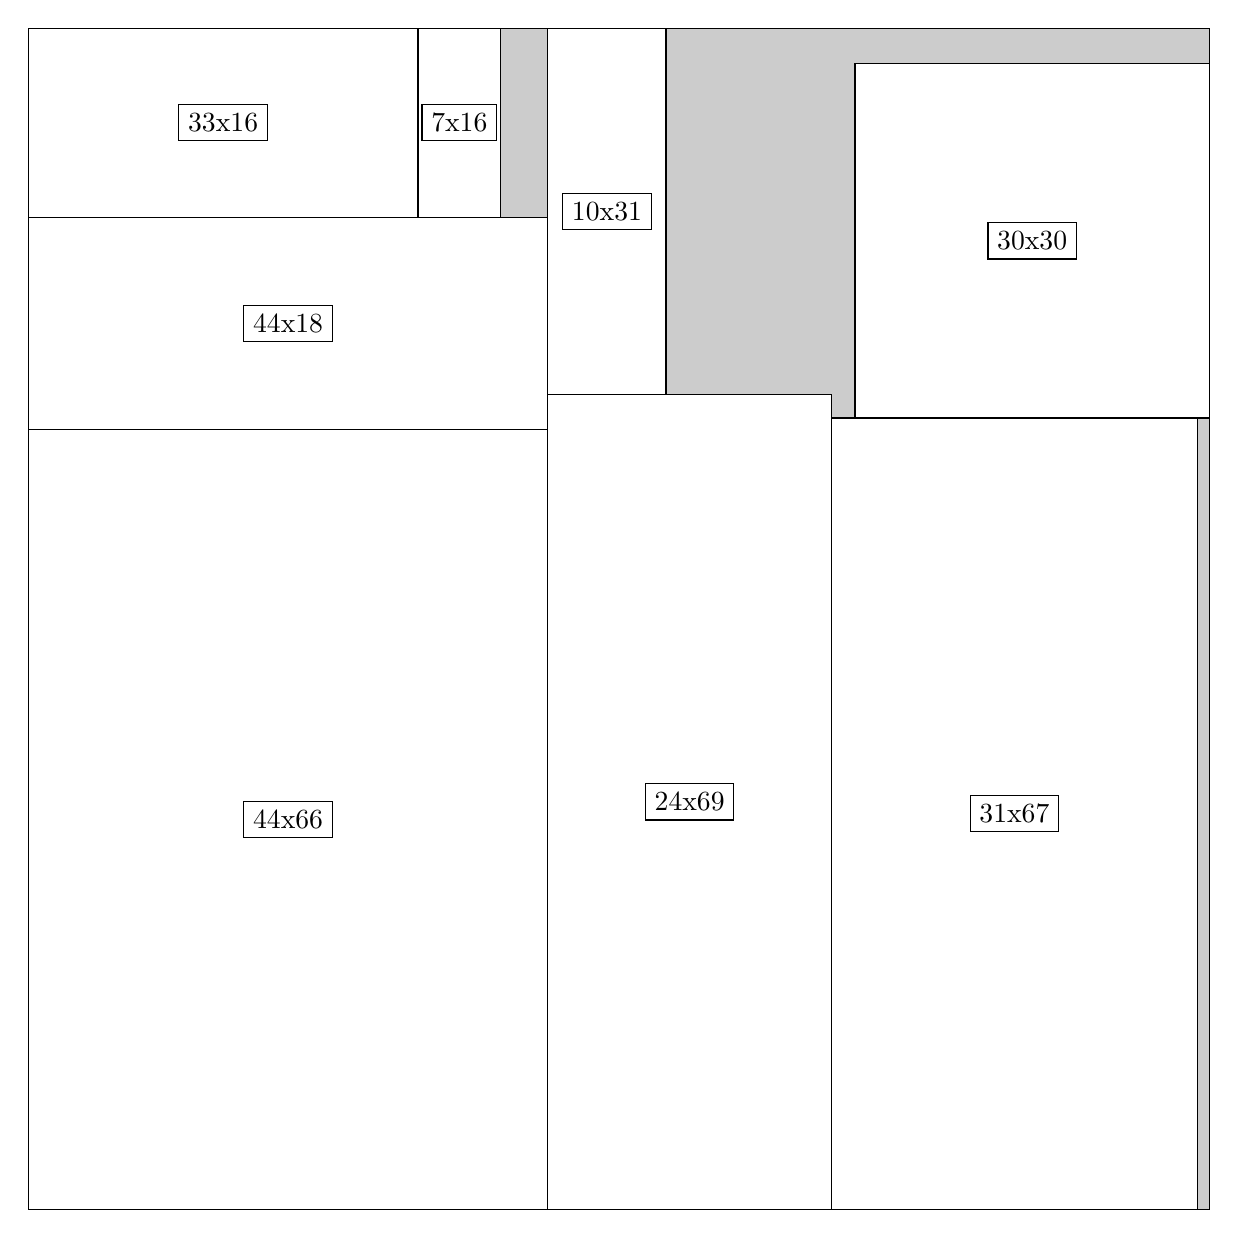
\begin{tikzpicture}[shorten >=1pt,scale=1.0,every node/.style={scale=1.0},->]
\tikzstyle{vertex}=[circle,fill=black!25,minimum size=14pt,inner sep=0pt]
\filldraw[fill=gray!40!white, draw=black] (0,0) rectangle (15.0,15.0);
\foreach \name/\x/\y/\w/\h in {44x66/0.0/0.0/6.6/9.9,24x69/6.6/0.0/3.5999999999999996/10.35,31x67/10.2/0.0/4.6499999999999995/10.049999999999999,30x30/10.5/10.049999999999999/4.5/4.5,44x18/0.0/9.9/6.6/2.6999999999999997,33x16/0.0/12.6/4.95/2.4,10x31/6.6/10.35/1.5/4.6499999999999995,7x16/4.95/12.6/1.05/2.4}
\filldraw[fill=white!40!white, draw=black] (\x,\y) rectangle node[draw] (\name) {\name} ++(\w,\h);
\end{tikzpicture}


w =44 , h =66 , x =0 , y =0 , v =2904
\par
w =24 , h =69 , x =44 , y =0 , v =1656
\par
w =31 , h =67 , x =68 , y =0 , v =2077
\par
w =30 , h =30 , x =70 , y =67 , v =900
\par
w =44 , h =18 , x =0 , y =66 , v =792
\par
w =33 , h =16 , x =0 , y =84 , v =528
\par
w =10 , h =31 , x =44 , y =69 , v =310
\par
w =7 , h =16 , x =33 , y =84 , v =112
\par
\newpage


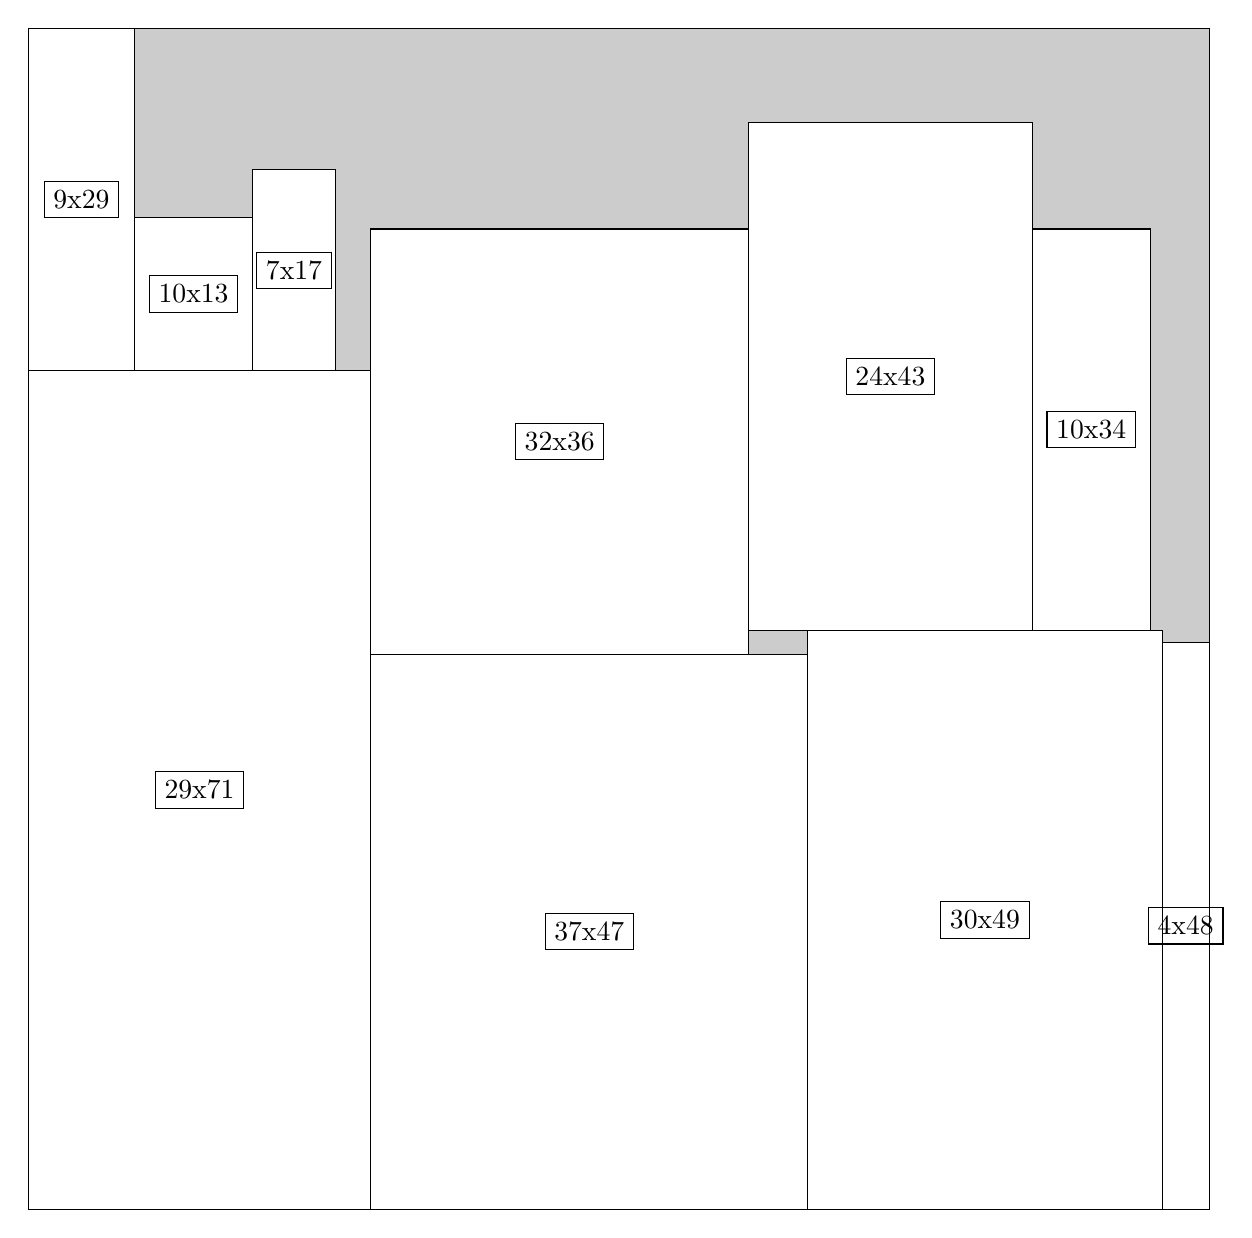
\begin{tikzpicture}[shorten >=1pt,scale=1.0,every node/.style={scale=1.0},->]
\tikzstyle{vertex}=[circle,fill=black!25,minimum size=14pt,inner sep=0pt]
\filldraw[fill=gray!40!white, draw=black] (0,0) rectangle (15.0,15.0);
\foreach \name/\x/\y/\w/\h in {29x71/0.0/0.0/4.35/10.65,37x47/4.35/0.0/5.55/7.05,30x49/9.9/0.0/4.5/7.35,32x36/4.35/7.05/4.8/5.3999999999999995,24x43/9.15/7.35/3.5999999999999996/6.45,10x34/12.75/7.35/1.5/5.1,9x29/0.0/10.65/1.3499999999999999/4.35,4x48/14.399999999999999/0.0/0.6/7.199999999999999,10x13/1.3499999999999999/10.65/1.5/1.95,7x17/2.85/10.65/1.05/2.55}
\filldraw[fill=white!40!white, draw=black] (\x,\y) rectangle node[draw] (\name) {\name} ++(\w,\h);
\end{tikzpicture}


w =29 , h =71 , x =0 , y =0 , v =2059
\par
w =37 , h =47 , x =29 , y =0 , v =1739
\par
w =30 , h =49 , x =66 , y =0 , v =1470
\par
w =32 , h =36 , x =29 , y =47 , v =1152
\par
w =24 , h =43 , x =61 , y =49 , v =1032
\par
w =10 , h =34 , x =85 , y =49 , v =340
\par
w =9 , h =29 , x =0 , y =71 , v =261
\par
w =4 , h =48 , x =96 , y =0 , v =192
\par
w =10 , h =13 , x =9 , y =71 , v =130
\par
w =7 , h =17 , x =19 , y =71 , v =119
\par
\newpage


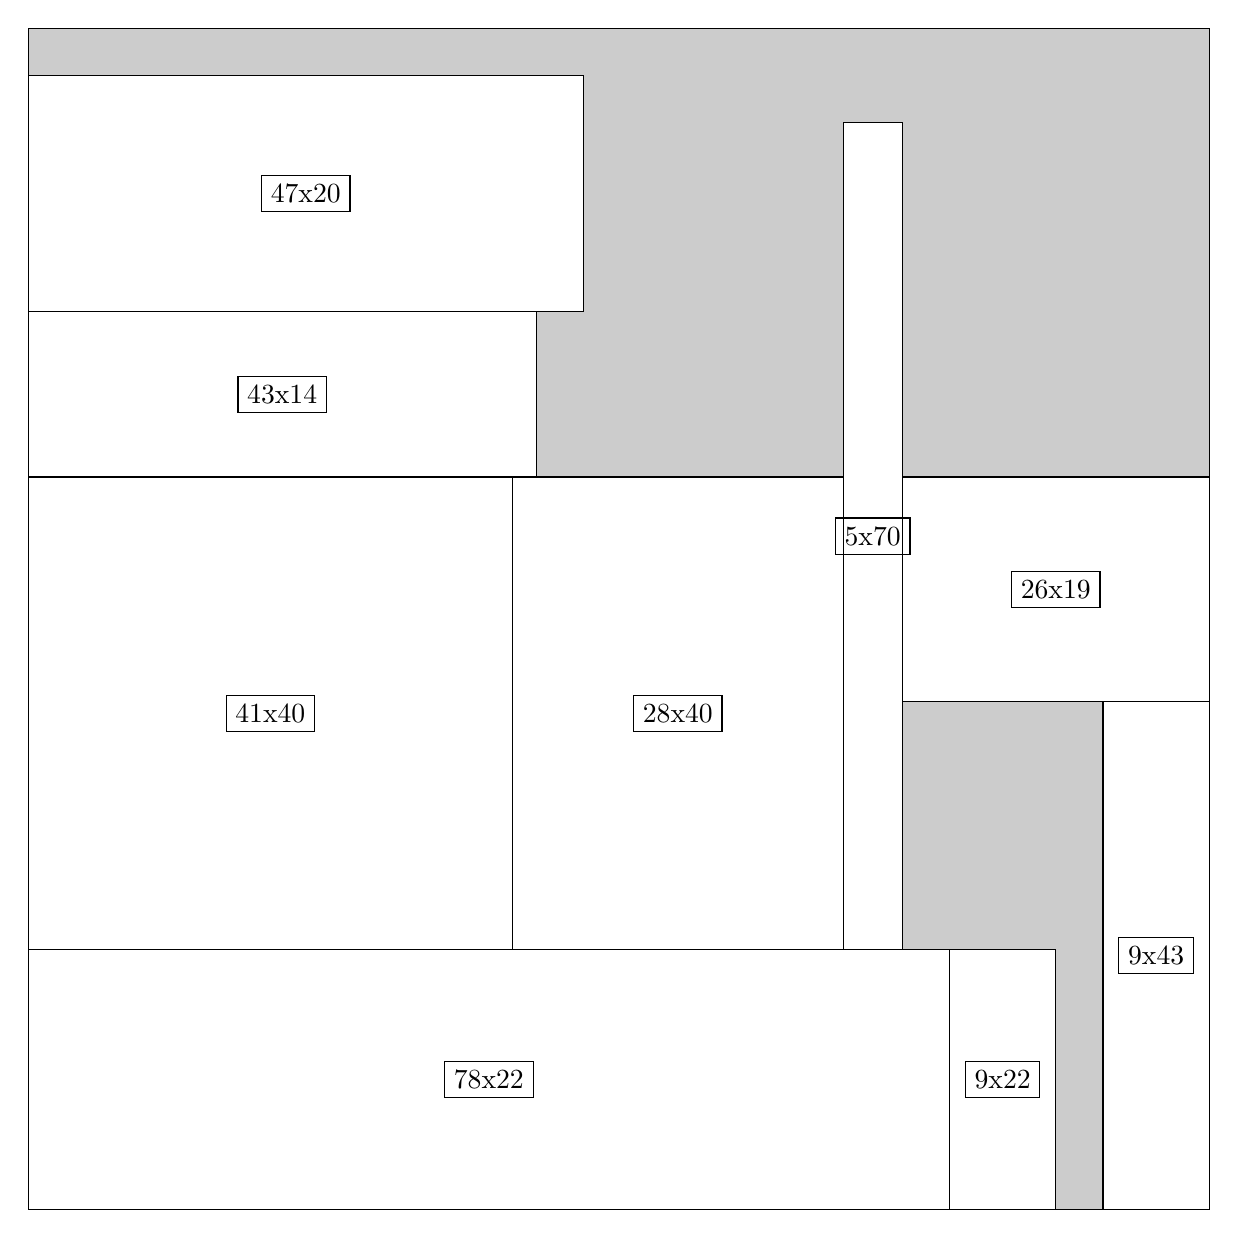
\begin{tikzpicture}[shorten >=1pt,scale=1.0,every node/.style={scale=1.0},->]
\tikzstyle{vertex}=[circle,fill=black!25,minimum size=14pt,inner sep=0pt]
\filldraw[fill=gray!40!white, draw=black] (0,0) rectangle (15.0,15.0);
\foreach \name/\x/\y/\w/\h in {78x22/0.0/0.0/11.7/3.3,41x40/0.0/3.3/6.1499999999999995/6.0,28x40/6.1499999999999995/3.3/4.2/6.0,47x20/0.0/11.4/7.05/3.0,43x14/0.0/9.299999999999999/6.45/2.1,26x19/11.1/6.45/3.9/2.85,9x43/13.65/0.0/1.3499999999999999/6.45,5x70/10.35/3.3/0.75/10.5,9x22/11.7/0.0/1.3499999999999999/3.3}
\filldraw[fill=white!40!white, draw=black] (\x,\y) rectangle node[draw] (\name) {\name} ++(\w,\h);
\end{tikzpicture}


w =78 , h =22 , x =0 , y =0 , v =1716
\par
w =41 , h =40 , x =0 , y =22 , v =1640
\par
w =28 , h =40 , x =41 , y =22 , v =1120
\par
w =47 , h =20 , x =0 , y =76 , v =940
\par
w =43 , h =14 , x =0 , y =62 , v =602
\par
w =26 , h =19 , x =74 , y =43 , v =494
\par
w =9 , h =43 , x =91 , y =0 , v =387
\par
w =5 , h =70 , x =69 , y =22 , v =350
\par
w =9 , h =22 , x =78 , y =0 , v =198
\par
\newpage


\end{document}